\section{逐项读懂现有图表与实际实验结果}\label{sec:results}
\subsection{先确认实验规模，再看小数点}
GBM 的正式路径数为 $160000$，独立控制变量预实验为 $20000$ 条；最细网格为 $1024$ 步。
生产种子为 $2026090804$，预实验种子为 $2026090805$，批大小为 $2000$。
强阶和控制后弱阶的主要拟合窗口为 $N=64,128,256,512,1024$。

非仿射模型使用 $100000$ 条路径，生产种子为 $2026090804$，批大小为 $512$，最细参考为 $8192$ 步。
两个模型是\emph{两个独立设计的实验}；使用相同种子并不使它们构成逐路径的模型对照。
原始摘要记录的 GBM 和非仿射实验耗时分别约为 $30.88$ 秒和 $107.80$ 秒，后者另记 JIT 预热；
这些是原运行环境的历史记录，不是本次机器的性能测试，也不是保证任何电脑都能达到的速度。

\subsection{GBM 强误差：数值体现了什么？}
表~\ref{tab:results-gbm-strong} 列出全部网格的强误差。
横向比较可见，同一步长下 Milstein 的平均路径误差明显更小；纵向比较则回答误差怎样随步长下降。
\begin{table}[htbp]\centering\small
\caption{GBM 的终值强误差。半宽指 95\% 蒙特卡洛区间半宽；正式路径数为 160000。}\label{tab:results-gbm-strong}
\begin{tabular}{rrrrr}\toprule
$N$ & EM 强误差 & 区间半宽 & Milstein 强误差 & 区间半宽\\\midrule
8 & 1.847500 & 0.008087 & 0.171271 & 0.001004\\
16 & 1.322183 & 0.005618 & 0.090960 & 0.000479\\
32 & 0.938467 & 0.003956 & 0.046965 & 0.000232\\
64 & 0.666408 & 0.002783 & 0.023908 & 0.000114\\
128 & 0.470714 & 0.001959 & 0.012093 & 0.000057\\
256 & 0.332966 & 0.001387 & 0.006096 & 0.000028\\
512 & 0.235503 & 0.000979 & 0.003060 & 0.000014\\
1024 & 0.166581 & 0.000693 & 0.001533 & 0.000007\\
\bottomrule
\end{tabular}
\end{table}


在主窗口上的拟合斜率为
\begin{equation}\label{eq:results-gbm-rates}
 \widehat p_{E}=0.49994677,\qquad \widehat p_M=0.99091845.
\end{equation}
以 EM 为例，从 $N=64$ 到 $N=1024$，步长缩小 $16$ 倍；若是半阶，误差应缩小 $\sqrt{16}=4$ 倍。
实际误差从 $0.666408$ 降到 $0.166581$，十分接近这一关系。
Milstein 同期从 $0.023908$ 降到 $0.001533$，缩小约 $15.60$ 倍，接近一阶预期的 $16$ 倍。
误差单位是价格单位；这些数是终值平均绝对差，不是百分比，也不是最大损失。

\begin{figure}[htbp]\centering
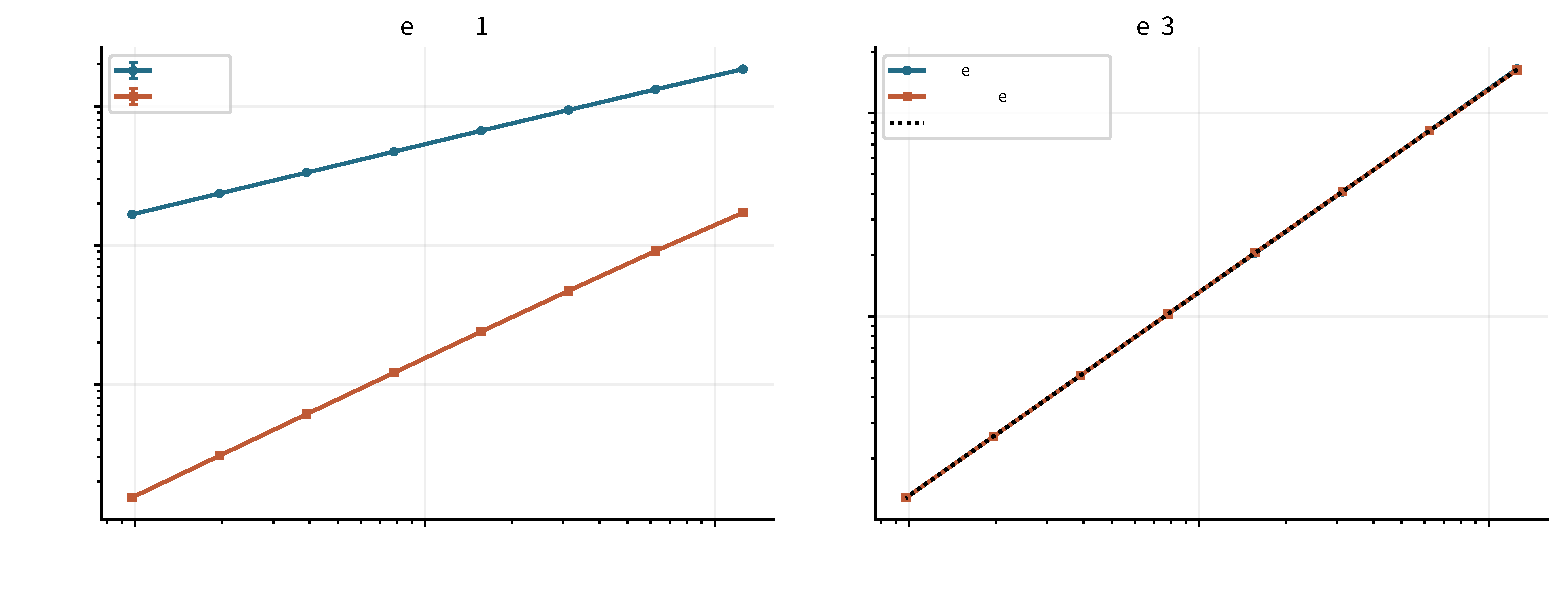
\includegraphics[width=\textwidth]{assets/gbm_results_zh.pdf}
\caption{由现有 CSV 重绘的 GBM 收敛图。左图的误差棒是逐点 95\% 采样区间；右图的三个趋势几乎重合，其精细差异需要结合数值表与区间阅读。}\label{fig:results-gbm}
\end{figure}
图~\ref{fig:results-gbm} 左图的纵轴跨多个数量级，便于看斜率。
斜率接近理论值是算法和实验设计正确的证据，但一张有限样本图不能代替一般收敛定理的证明。

\begin{figure}[htbp]\centering
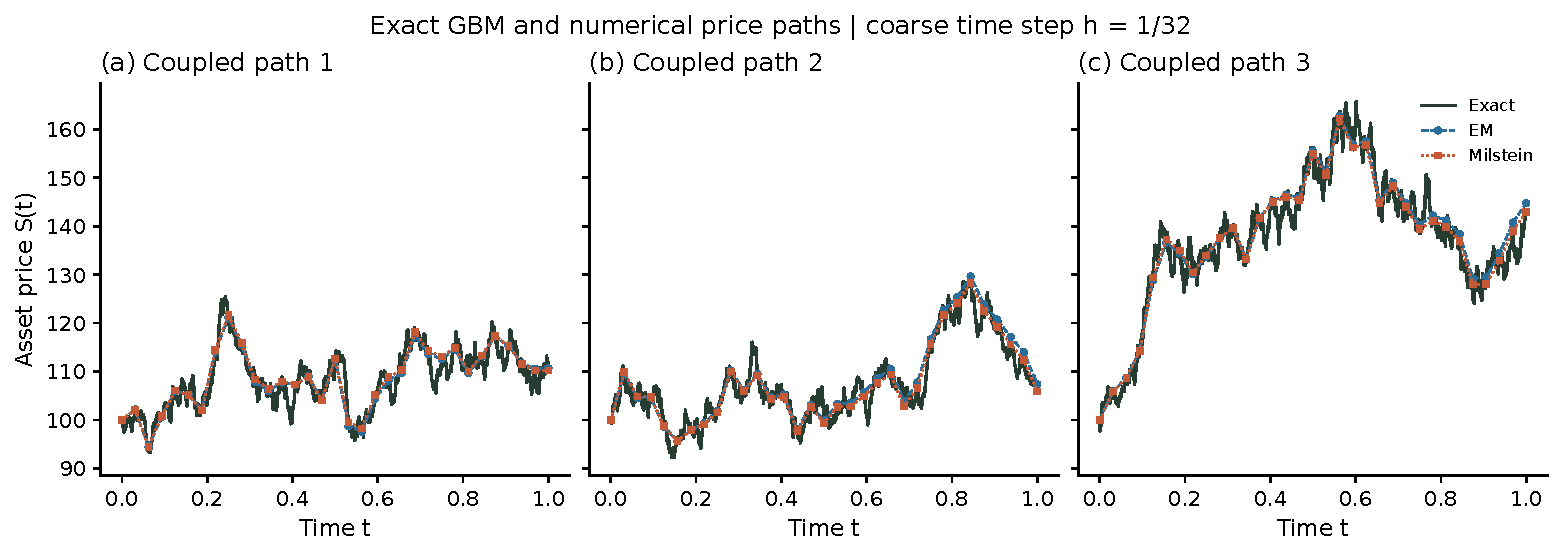
\includegraphics[width=\textwidth]{assets/gbm_paths.pdf}
\caption{原项目的三条共同驱动 GBM 示例路径。Exact 表示精确网格值，EM 与 Milstein 表示价格离散法；粗步长为 $1/32$。横轴是时间，纵轴是价格。}\label{fig:results-paths}
\end{figure}
图~\ref{fig:results-paths} 适合建立“沿同一随机路径逼近”的直觉。
三条样本路径不足以估计收敛阶，而且示例图使用独立于正式实验的随机种子；正式结论来自表~\ref{tab:results-gbm-strong} 的大规模统计。

\subsection{GBM 弱偏差：两种方法为什么几乎一样？}
表~\ref{tab:results-gbm-weak} 将实际控制后估计和解析偏差并列。
两种方法理论均值相同，故该观测量的真偏差相同；模拟值的末位差异来自残余抽样波动。
\begin{table}[htbp]\centering\small
\caption{GBM 的有符号均值偏差：数值减精确。控制后结果仍是模拟估计，解析列是独立核对目标。}\label{tab:results-gbm-weak}
\begin{tabular}{rrrr}\toprule
$N$ & 解析偏差（两方法） & EM 控制后估计 & Milstein 控制后估计\\\midrule
8 & -0.01635672 & -0.01649334 & -0.01629237\\
16 & -0.00819567 & -0.00821180 & -0.00818854\\
32 & -0.00410218 & -0.00409560 & -0.00410591\\
64 & -0.00205218 & -0.00204654 & -0.00205508\\
128 & -0.00102636 & -0.00102512 & -0.00102700\\
256 & -0.00051325 & -0.00051336 & -0.00051318\\
512 & -0.00025664 & -0.00025671 & -0.00025659\\
1024 & -0.00012832 & -0.00012836 & -0.00012831\\
\bottomrule
\end{tabular}
\end{table}

控制后的主窗口斜率分别约为 $0.99874039$ 和 $1.00039041$；解析偏差在全部八个网格上的拟合斜率为 $0.99926631$。
解析曲线并非在所有有限步长上严格等于 $Ch$，还有高阶项，因此有限窗口斜率不必恰好为 1。

最细网格给出一个特别清楚的统计例子：EM 解析偏差为 $-0.0001283247$，
控制后估计为 $-0.0001283595$，95\% 区间为约
$[-0.0001285244,-0.0001281946]$，包含解析目标。
未经控制的配对 EM 区间却跨过零，甚至点估计符号为正。
改善的是估计精度，而不是把 EM 更新公式改成了另一种算法。
Milstein 在最细网格的原始配对区间已经不含零，不能笼统认为所有未经控制的估计都无法分辨偏差。

\subsection{分布图：精确模拟也会与理论曲线有差别}
表~\ref{tab:results-quantiles} 给出 $h=1/8$ 时的分位数；这里用较粗网格使离散差异更容易观察。
\begin{table}[htbp]\centering\small
\caption{GBM 在粗网格 $h=1/8$ 上的分位数。精确模拟列也具有有限样本波动。}\label{tab:results-quantiles}
\begin{tabular}{rrrrr}\toprule
概率 $p$ & 理论分位数 & 精确模拟 & EM & Milstein\\\midrule
0.001 & 39.770 & 39.916 & 37.544 & 40.302\\
0.01 & 50.012 & 49.928 & 48.387 & 50.213\\
0.05 & 61.357 & 61.378 & 60.512 & 61.615\\
0.25 & 82.091 & 82.151 & 82.303 & 82.263\\
0.5 & 100.501 & 100.557 & 101.088 & 100.582\\
0.75 & 123.041 & 123.164 & 123.653 & 123.057\\
0.95 & 164.618 & 164.485 & 163.370 & 164.043\\
0.99 & 201.961 & 202.402 & 198.376 & 201.539\\
0.999 & 253.976 & 256.942 & 247.089 & 255.780\\
\bottomrule
\end{tabular}
\end{table}

例如理论 $1\%$ 分位数约为 $50.012$，EM 为 $48.387$，Milstein 为 $50.213$。
理论 $99\%$ 分位数约为 $201.961$，EM 为 $198.376$，Milstein 为 $201.539$。
这展示了均值以外的分布特征；不同位置不保证每次都按同样顺序接近理论值。

\begin{figure}[htbp]\centering
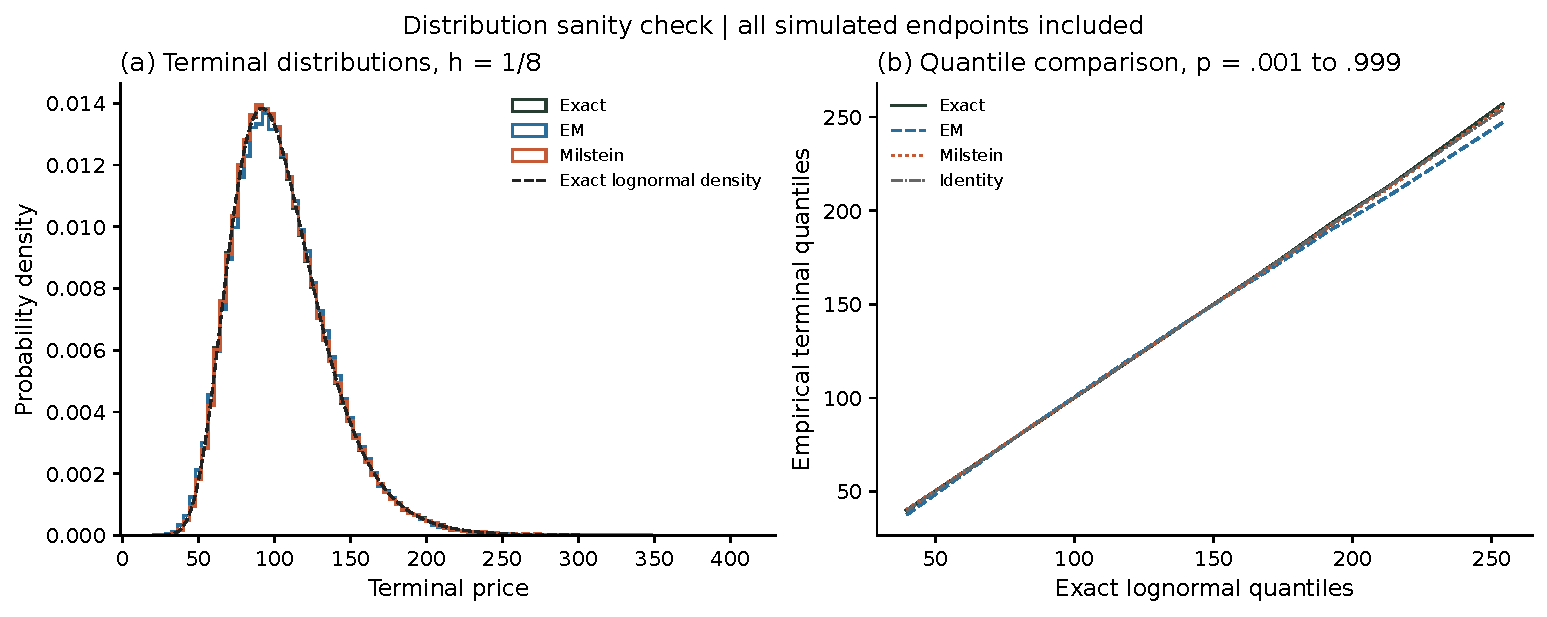
\includegraphics[width=\textwidth]{assets/gbm_distribution.pdf}
\caption{原项目的终值分布图。左图横轴为终值价格，纵轴为密度；右图横轴为理论对数正态分位数，纵轴为经验分位数。Identity 是两者完全相等的参考线。}\label{fig:results-distribution}
\end{figure}
图~\ref{fig:results-distribution} 中即使 Exact 曲线也不会与理论曲线处处重合，因为它来自有限个精确样本。
尾部更容易有较大的采样波动。例如 $0.1\%$ 尾部在 $160000$ 条路径中只有约 $160$ 个观测，极端分位数自然不如中位数稳定。
不能把精确样本与理论分位数之间的每一点差都归咎于时间离散。

\subsection{非仿射强差与弱差：哪些结论已得到支持？}
表~\ref{tab:results-na} 的参考统一为 $8192$ 步。
主强阶窗口是 $N=8,16,32,64$，斜率约为 $0.49145004$。
它支持“该窗口内表现与半阶相容”的判断；由于参考是数值解，应称\emph{经验强阶}。
\begin{table}[htbp]\centering\small
\caption{非仿射模型相对 8192 步参考的结果。100000 条共同路径；区间只量化配对弱差的抽样不确定性。}\label{tab:results-na}
\begin{tabular}{rrrr}\toprule
粗步数 $N$ & 终值强差 & 有符号收益差 & 收益差 95\% 区间\\\midrule
8 & 1.253542 & 0.025793 & $[0.016721,\ 0.034864]$\\
16 & 0.900872 & 0.010477 & $[0.004046,\ 0.016908]$\\
32 & 0.638177 & 0.005402 & $[0.000891,\ 0.009914]$\\
64 & 0.451761 & 0.001722 & $[-0.001479,\ 0.004923]$\\
128 & 0.318537 & 0.000959 & $[-0.001302,\ 0.003220]$\\
256 & 0.223226 & 0.000339 & $[-0.001243,\ 0.001922]$\\
\bottomrule
\end{tabular}
\end{table}


\begin{figure}[htbp]\centering
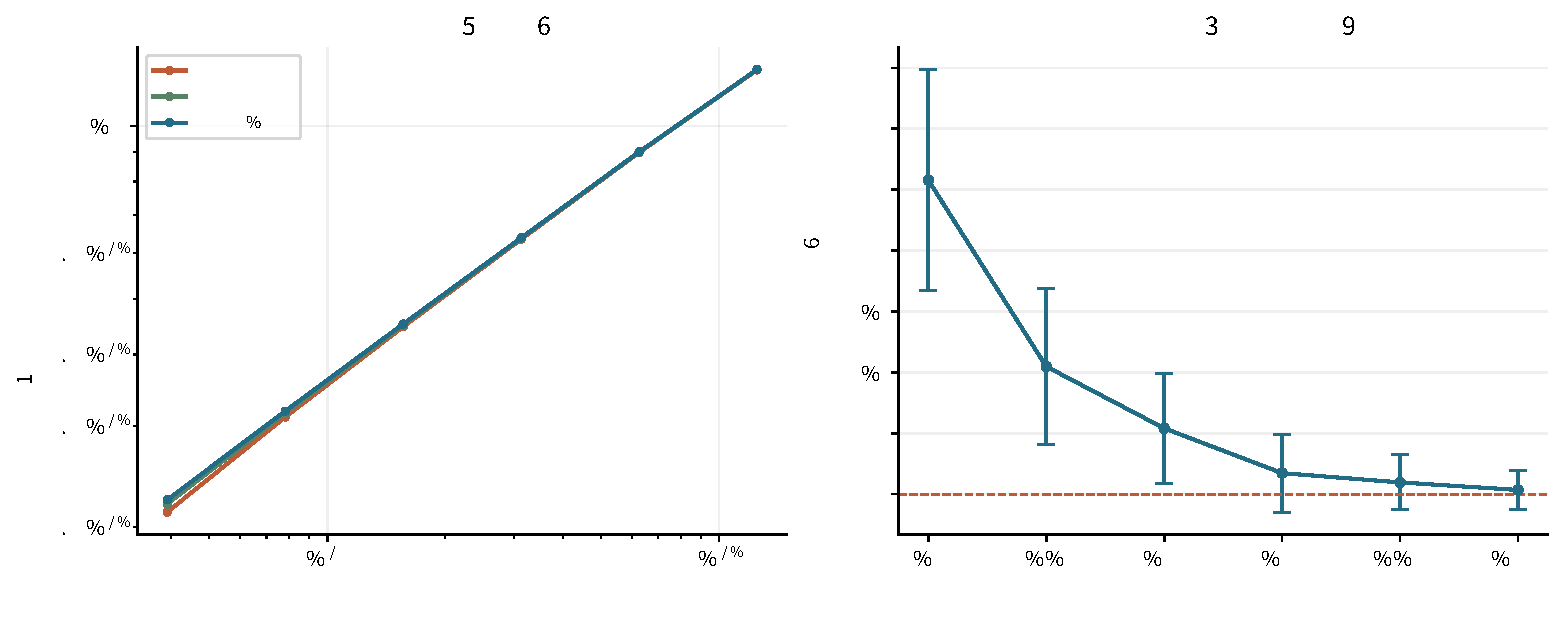
\includegraphics[width=\textwidth]{assets/nonaffine_results_zh.pdf}
\caption{现有非仿射结果的中文重绘。左图比较三层参考；右图保留收益偏差符号及采样区间，能直接看到后三个粗网格的区间跨过零。}\label{fig:results-na}
\end{figure}
图~\ref{fig:results-na} 左图的三条曲线很接近，但更细粗网格处参考影响的\emph{相对}比例增大。
右图前三个点的收益差为正，区间不含零；从 $N=64$ 起区间跨零。
因此当前数据能看到若干粗网格存在可分辨的收益差，却不足以在整个区间上宣称弱一阶。
这不是“实验失败”，而是统计实验对可支持结论作出的边界判断。

最细参考的价格均值为 $105.08796$。其 95\% 区间是 $[104.89962,105.27629]$，包含理论均值 $105.12711$。
但按式~\eqref{eq:ref-discrete-mean}，所有步长都能在期望上匹配这一均值，因此该检查只能作为有限的实现核对。

\subsection{参考加密与驱动检查：不能省掉的配套证据}
表~\ref{tab:results-reference} 显示两个相邻参考差。
收益差很小、区间跨零，说明当前样本没有明显分辨它的符号；强差则仍明显非零。
“收益均值几乎一致”和“同路径终值仍有差异”可以同时成立。
\begin{table}[htbp]\centering\small
\caption{相邻参考网格之间的差。收益差按较粗参考减较细参考计算。}\label{tab:results-reference}
\begin{tabular}{lrrr}\toprule
参考步数加密 & 平均绝对差 & 收益均值差 & 收益差 95\% 区间\\\midrule
2048$\to$4096 & 0.05679005 & -0.00002289 & $[-0.0004228,\ 0.0003770]$\\
4096$\to$8192 & 0.04015705 & 0.00009423 & $[-0.0001879,\ 0.0003763]$\\
\bottomrule
\end{tabular}
\end{table}


非仿射程序在事先指定的第一个批次检验布朗增量，共 $8192\times512=4194304$ 对。
每个增量方差的目标是 $1/8192=0.0001220703125$，实测约为 $0.00012207933$ 与 $0.00012208819$；
实测相关系数约为 $-0.69967521$，目标是 $-0.7$。
这是生成数据后的样本检查，不能只把公式写对就宣称数据诊断已经做过。
它使用第一批增量，并非全部 $100000$ 条路径的所有增量。

状态检查遍历全部网格更新：总更新次数为 $1484000000$。
最细网格保存的 $X$ 极值约为 $2.9739$ 与 $5.6969$，$Y$ 极值约为 $-2.8304$ 与 $1.8819$。
这些 $Y$ 的负值合法；程序报告所有中间 $X,Y$ 有限，并通过指数范围检查。

\subsection{本次独立复核覆盖了什么？}
新增 \texttt{audit\_saved\_results.py} 直接读取原 NPZ、CSV、JSON，独立重算可从终值恢复的统计量。
输出 \texttt{validation\_saved.json} 为 PASS。
它核对 GBM 保存的粗细层强误差、原始配对均值差、分位数和矩公式，以及非仿射的全部 18 组粗参考比较、2 组参考加密、9 层终值与收益统计和强阶拟合。

原保存文件没有储存全部布朗增量和正式控制变量，所以仅靠终值数组无法独立重算控制后的 GBM 弱偏差，也无法重算历史的中间状态检查。
这些部分分别依靠公式与代码审读，以及原运行保存的诊断记录。
本次没有直接运行依赖 Numba 的原 \texttt{verify.py} 内核检查，也没有重新仿真全部大型路径。
教学脚本的确定性检查与小规模运行已单独通过；它们是另一层实现核对，不能冒称重跑了原实验。
